

\chapter{Les technologies utilisées}

\section{Un bref historique du développement d'applications mobiles}
Le développement d'applications mobiles est l'acte ou le processus par lequel une application est développée pour les appareils mobiles. Ces applications peuvent être préinstallées sur les téléphones au cours de la fabrication ou accessibles via un navigateur Web \cite{noauthor_mobile_2019}. Toutefois, au cours de la dernière décennie \cite{leler_whats_2017}, des développeurs tiers ont été capables de créer des applications mobiles. Cependant, en raison de la concurrence intense dans les logiciels mobiles et des modifications apportées à chacune des plateformes, ces développeurs doivent prendre en compte un large éventail de tailles d'écran, de spécifications matérielles et de configurations.

Le développement d'applications mobiles est un domaine d'activité relativement récent. il n’est donc pas surprenant que les outils évoluent encore.
\newpage

\subsection{Les kits de développement de plate-forme (Platform SDKs)}
Le SDK Apple iOS est sorti en 2008 et le SDK Google Android en 2009. Ces deux SDK étaient basés sur des langages différents: Objective-C et Java, respectivement.
Votre application communique avec la plateforme pour créer des widgets ou accéder à des services tels que la caméra. Les widgets sont rendus dans un canevas d’écran et les événements sont renvoyés aux widgets. C'est une architecture simple, mais vous devez créer des applications séparées pour chaque plate-forme car les widgets sont différents, sans parler des langues natives\cite{leler_whats_2017}.

\begin{figure}[h]
	\begin{center}
		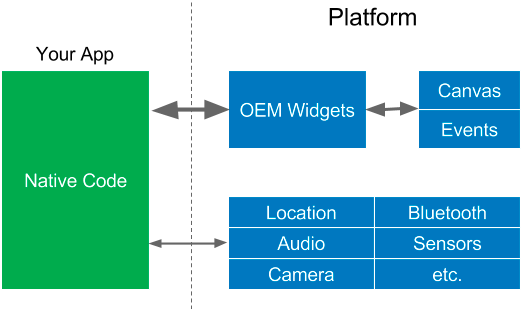
\includegraphics[width=10cm]{Images/chapter2/platform_sdk.png}
		\caption{{\footnotesize Architecture du développement mobile a l'aide des SDK\cite{leler_whats_2017}}}
	\end{center}
\end{figure}

\subsection{Vues Web (WebViews)}
Les premiers frameworks multi-plateformes étaient basés sur JavaScript et WebViews. Les exemples incluent une famille de frameworks liés: PhoneGap, Apache Cordova, Ionic, etc. Avant de publier leur SDK iOS, Apple avait encouragé les développeurs tiers à créer des applications Web pour iPhone. Il était donc évident de créer des applications multiplates-formes à l'aide de technologies Web.

\begin{figure}[h]
	\begin{center}
		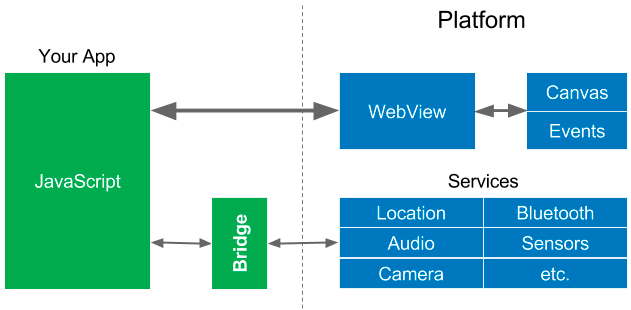
\includegraphics[width=11cm]{Images/chapter2/webview.png}
		\caption{{\footnotesize Architecture du développement mobile a l'aide des WebViews\cite{leler_whats_2017}}}
	\end{center}
\end{figure}

Votre application crée du HTML et l'affiche dans une vue Web sur la plateforme. Notez qu'il est difficile pour des langages tels que JavaScript de parler directement au code natif (comme les services), de sorte qu'ils passent par un «pont» qui fait que le contexte bascule entre le domaine JavaScript et le domaine natif. Comme les services de plate-forme ne sont généralement pas appelés très souvent, cela n’a pas causé trop de problèmes de performances\cite{leler_whats_2017}.

\subsection{Vues réactives (Reactive Views)}
Les infrastructures Web réactives telles que ReactJS (et d'autres) sont devenues populaires, principalement parce qu'elles simplifient la création de vues Web grâce à l'utilisation de modèles de programmation empruntés à la programmation réactive. En 2015, React Native a été créé pour apporter les nombreux avantages des vues réactives aux applications mobiles.\\

\begin{figure}[h]
	\begin{center}
		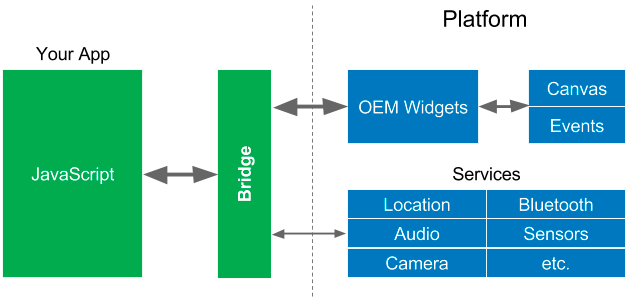
\includegraphics[width=11cm]{Images/chapter2/reactive_views.png}
		\caption{{\footnotesize Architecture du développement mobile a l'aide des Reactive Views\cite{leler_whats_2017}}}
	\end{center}
\end{figure}

\begin{wrapfigure}[8]{r}{2cm}
	
\includegraphics[width=2cm]{Images/chapter2/react_native_logo.png}
	\caption{{\footnotesize Logo de React Native}}
\end{wrapfigure}

React Native est très populaire (et mérite de l'être), mais comme le domaine JavaScript accède aux widgets de la plate-forme dans le domaine natif, il doit également passer par le pont. Les widgets sont généralement utilisés assez fréquemment (jusqu'à 60 fois par seconde lors d'animations, de transitions ou lorsque l'utilisateur balaie quelque chose sur l'écran avec son doigt), ce qui peut entraîner des problèmes de performances.

\section{Flutter}

\subsection{Qu'est-ce que Flutter?}

\begin{wrapfigure}[8]{r}{2cm}
	
\includegraphics[width=2cm]{Images/chapter2/flutter_logo.png}
	\caption{{\footnotesize Logo de Flutter}}
\end{wrapfigure}

Flutter est un SDK pour applications mobiles permettant de créer des applications hautes performances et haute fidélité pour iOS et Android à partir d'une seule base de code\cite{noauthor_technical_nodate}.\medskip

L'objectif est de permettre aux développeurs de proposer des applications hautes performances qui se sentent naturelles sur différentes plates-formes.

Nous adoptons des différences dans les comportements de défilement, la typographie, les icônes, etc.\bigskip

\begin{figure}[h]
	\begin{center}
		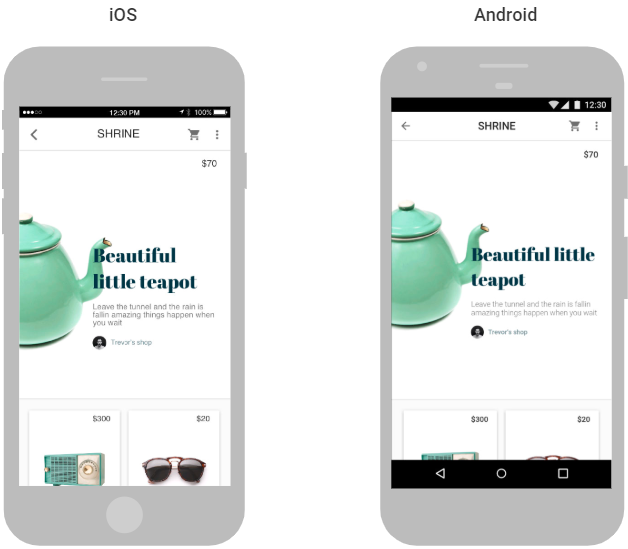
\includegraphics[width=9cm]{Images/chapter2/flutter_android_ios.png}
		\caption{{\footnotesize Ceci est une application de démonstration nommée Shrine\cite{noauthor_technical_nodate}}}
	\end{center}
\end{figure}

Comme React Native, Flutter fournit également des vues de style réactif. Flutter adopte une approche différente pour éviter les problèmes de performances causés par la nécessité d'un pont JavaScript en utilisant un langage de programmation compilé, à savoir Dart. Dart est compilé «à l'avance» \acrshort{AOT} en code natif pour plusieurs plates-formes. Cela permet à Flutter de communiquer avec la plate-forme sans passer par un pont JavaScript qui effectue un changement de contexte. La compilation en code natif améliore également les temps de démarrage des applications.\medskip

Flutter a une nouvelle architecture qui inclut des widgets qui ont l’air agréable, qui sont rapides, personnalisables et extensibles. il n'utilise pas les widgets de plate-forme (ou DOM WebViews), il fournit ses propres widgets.

\begin{figure}[h]
	\begin{center}
		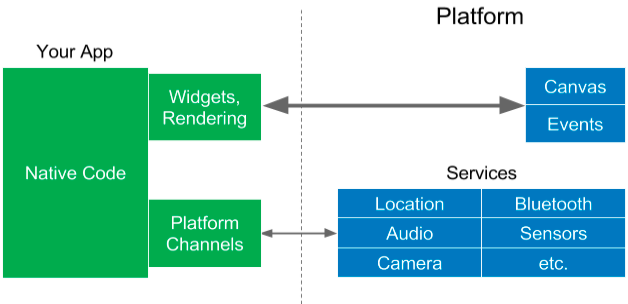
\includegraphics[width=11cm]{Images/chapter2/flutter.png}
		\caption{{\footnotesize Architecture du développement mobile a l'aide de Flutter\cite{leler_whats_2017}}}
	\end{center}
\end{figure}

Flutter soulève les widgets et le moteur de rendu de la plateforme dans l'application, ce qui leur permet d'être personnalisables et extensibles. Tout ce que Flutter a besoin de la plate-forme est un canevas dans lequel les widgets doivent être rendus afin qu’ils puissent apparaître sur l’écran du périphérique, ainsi que l’accès aux événements (touches, minuteries, etc.) et aux services (localisation, caméra, etc.).\medskip

Il existe toujours une interface entre le programme Dart (en vert) et le code de la plate-forme native (en bleu, pour iOS ou Android) qui effectue l’encodage et le décodage des données, mais cela peut être beaucoup plus rapide qu’un pont JavaScript.

\subsection{Principes de base}
Flutter comprend un \gls{framework} de style réact moderne, un moteur de rendu 2D, des widgets prêts à l'emploi et des outils de développement. Ces composants fonctionnent ensemble pour vous aider à concevoir, créer, tester et déboguer des applications. Tout est organisé autour de quelques principes fondamentaux.
\subsubsection{{\large 1 - Tout est un widget}}
Les widgets sont les éléments de base de l’interface utilisateur d’une application Flutter. Chaque widget est une déclaration immuable d'une partie de l'interface utilisateur. Contrairement aux autres frameworks qui séparent les vues, les contrôleurs de vue, les présentations et d'autres propriétés, Flutter possède un modèle objet cohérent et unifié: le widget.
Un widget peut définir:

\begin{list}{•}{}
	\item un élément structurel (comme un bouton ou un menu).
	\item un élément stylistique (comme une police ou un jeu de couleurs).
	\item un aspect de la mise en page (comme le rembourrage).
	\item etc…
\end{list}

Les widgets forment une hiérarchie basée sur la composition. Chaque widget niche à l'intérieur et hérite des propriétés de son parent. Il n'y a pas d'objet «application» séparé. Au lieu de cela, le widget racine joue ce rôle.
Vous pouvez répondre à des événements, comme une interaction utilisateur, en indiquant au cadre de remplacer un widget de la hiérarchie par un autre. La structure compare ensuite les nouveaux et les anciens widgets et met efficacement à jour l'interface utilisateur.\bigskip

\longtab \textbf{Composition> héritage\medskip}

Les widgets sont souvent eux-mêmes composés de nombreux petits widgets à usage unique qui se combinent pour produire des effets puissants. Par exemple, Container, un widget couramment utilisé, est composé de plusieurs widgets responsables de la mise en page, de la peinture, du positionnement et du dimensionnement. Plus précisément, Container est composé des widgets LimitedBox, ConstrainedBox, Align, Padding, DecoratedBox et Transform. Plutôt que de sous-classer Container pour produire un effet personnalisé, vous pouvez composer ces widgets simples, ainsi que d'autres, de manière innovante.\medskip

\begin{figure}[h]
	\begin{center}
		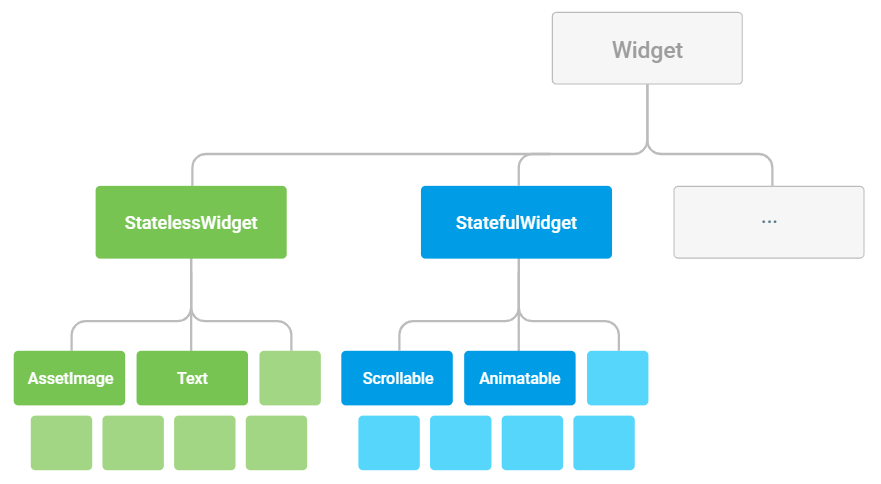
\includegraphics[width=13cm]{Images/chapter2/hierarchy_widgets.png}
		\caption{{\footnotesize Exemple d'une hierarchy des widgets\cite{noauthor_technical_nodate}}}
	\end{center}
\end{figure}

La hiérarchie des classes est peu profonde et large afin de maximiser le nombre possible de combinaisons.\medskip

Vous pouvez également contrôler la mise en page d'un widget en le composant avec d'autres widgets. Par exemple, pour centrer un widget, vous l'enroulez dans un widget Centre. Il existe des widgets pour le remplissage, l'alignement, les lignes, les colonnes et les grilles. Ces widgets de présentation ne possèdent pas de représentation visuelle. Au lieu de cela, leur seul objectif est de contrôler un aspect de la présentation d’un autre widget. Pour comprendre pourquoi un widget est rendu d’une certaine manière, il est souvent utile d’inspecter les widgets voisins.\bigskip

\longtab \textbf{Couches de framework Flutter\medskip}

Le framework Flutter est organisé en une série de couches, chaque couche s'appuyant sur la couche précédente.\medskip

\begin{figure}[h]
	\begin{center}
		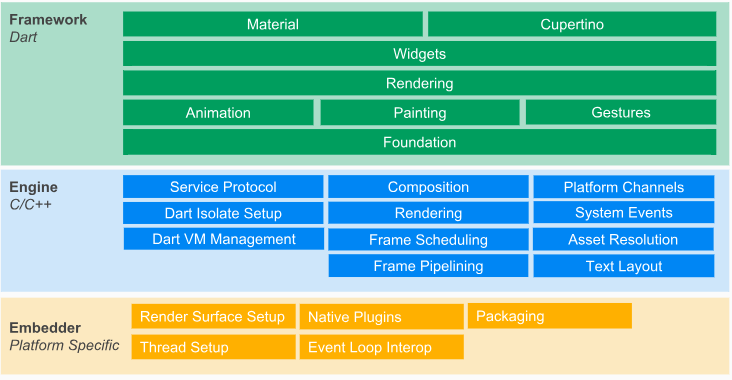
\includegraphics[width=13cm]{Images/chapter2/flutter_architecture.png}
		\caption{{\footnotesize L'architecture de flutter\cite{noauthor_technical_nodate}}}
	\end{center}
\end{figure}

Les couches supérieures du cadre sont utilisées plus fréquemment que les couches inférieures.\medskip

Le but de cette conception est de vous aider à faire plus avec moins de code. Par exemple, le calque Matérial est construit en composant les widgets de base à partir du calque Widgets, et le calque Widgets lui-même est construit en orchestrant des objets de niveau inférieur à partir du calque de rendu.
Les couches offrent de nombreuses options pour créer des applications.

Choisissez une approche personnalisée pour libérer toute la puissance d'expression du framework, ou utilisez des blocs de construction de la couche de widgets, ou combinez-les. Vous pouvez composer les widgets prêts à l'emploi fournis par Flutter ou créer vos propres widgets personnalisés à l'aide des mêmes outils et techniques que ceux utilisés par l'équipe Flutter pour créer le framework.

\subsubsection{{\large 2 - La construction de widgets}}
Vous définissez les caractéristiques uniques d'un widget en implémentant une fonction de génération qui renvoie une arborescence (ou une hiérarchie) de widgets. Cet arbre représente la partie de l’interface utilisateur du widget de manière plus concrète. Par exemple, un widget de barre d'outils peut avoir une fonction de génération qui renvoie une disposition horizontale de texte et de divers boutons. Le framework demande ensuite de manière récursive à chacun de ces widgets de construire jusqu'à ce que le processus se transforme en widgets entièrement concrets, que le framework assemble ensuite en un arbre.\medskip

La fonction de génération d’un widget doit être exempte d’effets secondaires. À chaque fois qu'il est invité à construire, le widget doit renvoyer une nouvelle arborescence de widgets, quel que soit ce que le widget a précédemment renvoyé. Le cadre fait beaucoup pour comparer la version précédente à la version actuelle et pour déterminer les modifications à apporter à l'interface utilisateur.\medskip

Cette comparaison automatisée est assez efficace, permettant des applications interactives hautes performances. Et la conception de la fonction de construction simplifie votre code en vous concentrant sur la déclaration d'un widget, plutôt que sur la complexité de la mise à jour de l'interface utilisateur d'un état à un autre.

\subsubsection{{\large 3 - Gestion de l'interaction utilisateur}}
Si les caractéristiques uniques d'un widget doivent être modifiées en fonction de l'interaction de l'utilisateur ou d'autres facteurs, ce widget est avec état. Par exemple, si un widget a un compteur qui s'incrémente chaque fois que l'utilisateur appuie sur un bouton, la valeur du compteur correspond à l'état de ce widget.\medskip
 
Lorsque cette valeur change, le widget doit être reconstruit pour mettre à jour l'interface utilisateur.\medskip

\begin{figure}[h]
	\begin{center}
		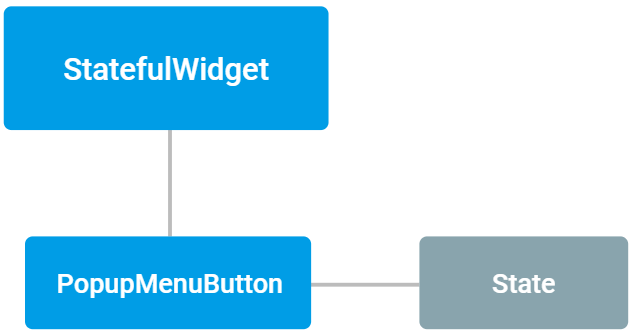
\includegraphics[width=10cm]{Images/chapter2/user_interaction_graph.png}
		\caption{{\footnotesize Modele d'une Widget Stateful\cite{noauthor_technical_nodate}}}
	\end{center}
\end{figure}

Ces widgets sous-classent StatefulWidget (plutôt que StatelessWidget) et stockent leur état mutable dans une sous-classe d’État.\medskip

Chaque fois que vous modifiez un objet State (par exemple, incrémentez le compteur), vous devez appeler setState() pour indiquer au framework de mettre à jour l'interface utilisateur en appelant à nouveau la méthode de compilation de State.\medskip

Avoir des objets state et widget séparés permet à d'autres widgets de traiter les widgets sans état et avec état de la même manière, sans craindre de perdre un état. Plutôt que de devoir conserver un enfant pour préserver son état, le parent est libre de créer une nouvelle instance de l'enfant sans perdre son état persistant. La structure fait tout le travail de recherche et de réutilisation des objets d'état existants, le cas échéant.


\subsection{Pourquoi utiliser Flutter?}
Comme nous l'avons mentionné précédemment, il existe de nombreuses options pour développer une application mobile, qu'il s'agisse de SDK natifs ou de frameworks multiplates-formes (Xamarin, ReactNative, Ionic, PhoneGap). Pour ce projet particulier, le framework Flutter a été choisi pour plusieurs points, dont les principaux sont:


\subsubsection{1. Multiplate-forme (cross-platform)}
Un produit ou système informatique multiplate-forme est un produit ou système pouvant fonctionner sur plusieurs types de plates-formes ou d'environnements d'exploitation.

Différents types de systèmes multiplates-formes incluent des systèmes matériels et logiciels, ainsi que des systèmes qui impliquent des versions séparées pour chaque plate-forme, ainsi que d'autres systèmes plus vastes conçus pour fonctionner de la même manière sur plusieurs plates-formes.
La plateforme croisée est également connue en tant que plate-forme indépendante\cite{noauthor_what_nodate}

Flutter offre la possibilité de créer une application compilée pour fonctionner à la fois sur Android et iOS à partir de la même base de code. Tout en maintenant l'expérience utilisateur appropriée sur chaque plate-forme.


\subsubsection{2. Productivité}
Flutter offre une augmentation de la productivité que provient du «rechargement à chaud» de Flutter («Stateful Hot Reload» et «Hot Restart». Ensemble, ils permettent aux développeurs de voir les modifications apportées à l'état d'une application en moins d'une seconde; structure de l'application en moins de dix.

Il n’est pas nécessaire d’exécuter une autre version de Gradle. Vous voyez vos modifications dès que vous enregistrez. Pour les développeurs, cela est souvent très facile à maîtriser - il n’ya que peu ou pas de courbe d’apprentissage liée à l’utilisation du «rechargement à chaud» car, par défaut, cela se produit chaque fois que vous enregistrez. Cependant, les avantages sont essentiels. Le temps de développement est souvent réduit de 30\% à 40\%, car les délais de reconstruction de Gradle qui ralentissent le développement des développeurs Android prennent généralement plus de temps à chaque modification appliquée.

\subsubsection{3. Intégration directe avec Firebase}
Firebase fournit un support prêt à l'emploi pour un ensemble de services tels que le stockage en nuage, les fonctions de nuage, les bases de données en temps réel, l'hébergement, l'authentification et bien plus encore. Votre infrastructure est instantanément sans serveur, redondante et évolutive. Cela signifie que vous n’avez pas à passer beaucoup de temps et de ressources à construire le backend. Il est également simple de le combiner avec un outil permettant d’automatiser votre processus de développement et de publication, tel que Fastlane; faciliter la livraison continue. Par conséquent, vous n'avez pas besoin de support DevOps dédié dans votre équipe.

\subsubsection{4. Performance}
L'application est compilée à l'avance en code ARM natif, pas au moment de l'exécution, comme dans React Native. Cela donne de meilleures performances car il n’ya pas de pont JS au milieu pour analyser et exécuter le code.

\subsubsection{5. L'utilisation de Dart}

\begin{wrapfigure}[7]{r}{5cm}
	
\includegraphics[width=5cm]{Images/chapter2/dart_logo.png}
	\caption{{\footnotesize Logo de Dart}}
\end{wrapfigure}

Dart est un langage de programmation polyvalent développé à l'origine par Google et ensuite approuvé en tant que norme par Ecma (ECMA-408). Il est utilisé pour créer des applications Web, serveur, bureau et mobiles.

Dart est un langage basé sur les objets, orienté objet, défini par la classe et utilisant une syntaxe de style C qui transcompile éventuellement en JavaScript. Il prend en charge les interfaces, mixins, classes abstraites, génériques réifiés, typage statique et un système de type sonore.\cite{noauthor_dart_2019}\medskip

Voici une liste rapide des fonctionnalités de Dart qui, ensemble, le rendent indispensable pour Flutter:

\begin{list}{•}{}
\item Dart est \acrshort{AOT} compilé en un code natif rapide et prévisible, qui permet à presque tout de Flutter d'être écrit en Dart. Cela rend non seulement Flutter rapide, mais pratiquement tout (y compris tous les widgets) peut être personnalisé.
\item Dart peut également être compilé \acrshort{JIT} (Just In Time) pour des cycles de développement exceptionnellement rapides et un flux de travail révolutionnaire (y compris le populaire rechargement à chaud avec état sous la seconde de Flutter).
\item Dart facilite la création d'animations lisses et de transitions exécutées à 60 images par seconde. Dart peut faire l’allocation d’objets et la collecte de place sans verrous. Et comme JavaScript, Dart évite la planification préemptive et la mémoire partagée (et donc les verrous). Les applications Flutter étant compilées en code natif, elles ne nécessitent pas de pont lent entre les domaines (par exemple, JavaScript vers natif). Ils démarrent aussi beaucoup plus vite.
\item Dart permet à Flutter d’éviter le recours à un langage de présentation déclaratif distinct, tel que \acrshort{JSX} ou \acrshort{XML}, ou à des générateurs d’interface visuelle distincts, car la présentation déclarative et programmatique de Dart est facile à lire et à visualiser. Et avec toute la mise en page dans une langue et à un endroit, il est facile pour Flutter de fournir des outils avancés qui facilitent la mise en page.
\item Les développeurs ont découvert que Dart est particulièrement facile à apprendre car il comporte des fonctionnalités bien connues des utilisateurs de langages statiques et dynamiques.
\end{list}

Toutes ces fonctionnalités ne sont pas propres à Dart, mais leur combinaison constitue un atout qui confère à Dart une puissance unique pour la mise en œuvre de Flutter. Tant pis, il est difficile d’imaginer que Flutter soit aussi puissant qu’il est sans Dart.\cite{leler_why_2018}


\section{Firebase}
\subsection{Introduction}

\begin{wrapfigure}[6]{r}{5cm}
	
\includegraphics[width=5cm]{Images/chapter2/firebase_logo.png}
	\caption{{\footnotesize Logo de Firebase}}
\end{wrapfigure}

Firebase est une plate-forme de développement d'applications mobiles et Web qui fournit aux développeurs une multitude d'outils et de services pour les aider à développer des applications de haute qualité, à développer leur base d'utilisateurs et à générer davantage de bénéfices.\cite{geekyants_introduction_2017}
\newpage

\subsection{Bref historique}
En 2011, avant que Firebase fût Firebase, c'était une startup appelée Envolve. En tant que Envolve, il fournissait aux développeurs une API qui permettait l'intégration de la fonctionnalité de discussion en ligne dans leur site Web.

Qu'est ce que c'est? Il est intéressant de noter que c'est utilisé pour envoyer des messages. Les développeurs utilisaient Envolve pour synchroniser les données des applications en tant qu'état de jeu en temps réel sur l'ensemble de leurs utilisateurs.

Ceci a conduit les fondateurs d’Envolve, James Tamplin et Andrew Lee, à séparer le système de chat et l’architecture en temps réel. En avril 2012, Firebase a été créée en tant que société distincte fournissant un système de gestion en temps réel.

Après son acquisition en 2014, Firebase a rapidement évolué pour devenir le monstre multifonctionnel d’une plate-forme mobile et Web qu’il est aujourd’hui.

\subsection{Les services de Firebase}
les services de Firebase peuvent être divisé en trois groupes:\bigskip\\
\longtab \textbf{1 - Construction des meilleures applications:}\bigskip

\begin{wrapfigure}[4]{l}{1cm}
	
\includegraphics[width=1cm]{Images/chapter2/firebase_services/firestore.png}
\end{wrapfigure}
\textbf{Firestore Cloud} Stockez et synchronisez des données entre utilisateurs et appareils - à l'échelle mondiale - à l'aide d'une base de données NoSQL hébergée dans le cloud. Cloud Firestore vous offre une synchronisation en direct et une assistance hors ligne, ainsi que des requêtes de données efficaces. Son intégration avec d'autres produits Firebase vous permet de créer de véritables applications sans serveur.\medskip

\begin{wrapfigure}[4]{l}{1cm}
	
\includegraphics[width=1cm]{Images/chapter2/firebase_services/mlkit.png}
\end{wrapfigure}
\textbf{Kit ML \textsuperscript{BETA} \acrshort{BETA}} Intégrez de puissantes fonctionnalités d'apprentissage automatique (Machine Learning) à votre application mobile, que vous soyez débutant ou expérimenté dans \acrshort{ML}. Commencez facilement en utilisant les API prêtes à l'emploi pour les cas d'utilisation courants des appareils mobiles ou importez vos propres modèles personnalisés qui peuvent être hébergés et fournis à vos applications par Firebase. Les API du kit ML peuvent s'exécuter sur le périphérique ou dans le cloud, en fonction des fonctionnalités. Certaines vous offrent les deux choix.\medskip\\

\begin{wrapfigure}[3]{l}{1cm}
	
\includegraphics[width=1cm]{Images/chapter2/firebase_services/cloud_function.png}
\end{wrapfigure}
\textbf{Fonctions Cloud} Étendez votre application avec du code d’arrière-plan personnalisé sans avoir à gérer et à faire évoluer vos propres serveurs. Les fonctions peuvent être déclenchées par des événements, émis par des produits Firebase, des services Google Cloud ou des tiers, à l'aide de \gls{Webhook}s.\medskip

\begin{wrapfigure}[4]{l}{1cm}
	
\includegraphics[width=1cm]{Images/chapter2/firebase_services/authentication.png}
\end{wrapfigure}
\textbf{Authentification} Gérez vos utilisateurs de manière simple et sécurisée. Firebase Auth propose plusieurs méthodes d’authentification, notamment un courrier électronique et un mot de passe, des fournisseurs tiers tels que Google ou Facebook et l’utilisation directe de votre système de compte existant. Construisez votre propre interface ou profitez de l'interface utilisateur open source entièrement personnalisable.\medskip

\begin{wrapfigure}[4]{l}{1cm}
	
\includegraphics[width=1cm]{Images/chapter2/firebase_services/hosting.png}
\end{wrapfigure}
\textbf{Hébergement} Simplifiez votre hébergement Web avec des outils spécialement conçus pour les applications Web modernes. Lorsque vous téléchargez vos ressources Web, ils seront automatiquement transféré vers le CDN mondial de la platforme Firebase et ils aient attribué un certificat SSL gratuit afin que vos utilisateurs bénéficient d'une expérience sécurisée, fiable et à faible latence, où qu'ils se trouvent.\medskip

\begin{wrapfigure}[4]{l}{1cm}
	
\includegraphics[width=1cm]{Images/chapter2/firebase_services/cloud_storage.png}
\end{wrapfigure}
\textbf{Stockage en ligne} Stockez et partagez des contenus générés par les utilisateurs, tels que des images, du son et de la vidéo, avec un stockage d’objets puissant, simple et économique, conçu à l’échelle de Google. Les SDK Firebase pour le stockage en nuage ajoutent la sécurité Google aux téléchargements de fichiers et aux téléchargements pour vos applications Firebase, quelle que soit la qualité du réseau.\medskip

\begin{wrapfigure}[4]{l}{1cm}
	
\includegraphics[width=1cm]{Images/chapter2/firebase_services/realtime_database.png}
\end{wrapfigure}
\textbf{Base de données en temps réel} Stockez et synchronisez les données entre les utilisateurs et les périphériques en temps réel à l'aide d'une base de données NoSQL hébergée dans le cloud. Les données mises à jour se synchronisent sur les appareils connectés en quelques millisecondes. Les données restent disponibles si votre application est déconnectée, offrant ainsi une expérience utilisateur exceptionnelle, quelle que soit la connectivité réseau.\bigskip

\longtab \textbf{2 - Amélioration de la qualité de l'application:}\bigskip

\begin{wrapfigure}[4]{l}{1cm}
	
\includegraphics[width=1cm]{Images/chapter2/firebase_services/crashlytics.png}
\end{wrapfigure}
\textbf{Crashlytics} Réduisez votre temps de dépannage en transformant une avalanche de collisions en une liste de problèmes gérables. Obtenez des informations claires et exploitables sur les problèmes à résoudre en premier en observant l'impact de l'utilisateur sur le tableau de bord de Crashlytics. Les alertes en temps réel vous aideront à rester au top de votre stabilité, même lors de vos déplacements. Crashlytics est le principal journaliste de crash pour Firebase.\medskip

\begin{wrapfigure}[3]{l}{1cm}
	
\includegraphics[width=1cm]{Images/chapter2/firebase_services/performance_monitoring.png}
\end{wrapfigure}
\textbf{Suivi de la performance} Diagnostiquez les problèmes de performances des applications survenant sur les appareils de vos utilisateurs. Utilisez des traces pour surveiller les performances de parties spécifiques de votre application et consultez une vue résumée de la console Firebase. Surveillez les heures de démarrage de votre application et surveillez les requêtes HTTP sans écrire de code.\medskip

\begin{wrapfigure}[4]{l}{1cm}
	
\includegraphics[width=1cm]{Images/chapter2/firebase_services/test_lab.png}
\end{wrapfigure}
\textbf{Laboratoire de test} Exécutez des tests automatiques et personnalisés pour votre application sur des périphériques virtuels et physiques hébergés par Google. Utilisez le laboratoire de test Firebase tout au long de votre cycle de développement pour détecter les bogues et les incohérences afin de pouvoir offrir une expérience inoubliable sur une grande variété de périphériques.\bigskip

\longtab \textbf{3 - Développement d'entreprise:}\bigskip

\begin{wrapfigure}[4]{l}{1cm}
	
\includegraphics[width=1cm]{Images/chapter2/firebase_services/in-app_messaging.png}
\end{wrapfigure}
\textbf{Messagerie In-App} Engagez et entretenez vos utilisateurs actifs avec des messages ciblés et contextuels qui les encouragent à effectuer des actions significatives au sein de votre application. Vous avez le pouvoir de déclencher des messages en fonction du comportement et des intérêts de l'utilisateur. Vous pouvez également personnaliser la conception des messages intégrés à votre marque. La messagerie in-app prend en charge un grand nombre de cas d'utilisation et de formats.\medskip

\begin{wrapfigure}[4]{l}{1cm}
	
\includegraphics[width=1cm]{Images/chapter2/firebase_services/google_analytics.png}
\end{wrapfigure}
\textbf{Google Analytics} Analysez les attributions et les comportements des utilisateurs dans un seul tableau de bord pour prendre des décisions éclairées concernant votre feuille de route. Obtenez des informations en temps réel à partir des rapports ou exportez vos données d'événements brutes vers Google BigQuery pour une analyse personnalisée.\medskip

\begin{wrapfigure}[4]{l}{1cm}
	
\includegraphics[width=1cm]{Images/chapter2/firebase_services/predictions.png}
\end{wrapfigure}
\textbf{Prédictions} Exploitez toute la puissance de l’apprentissage automatique de Google pour avoir une idée des segments d’utilisateurs susceptibles d’abandonner ou de dépenser (ou de terminer un autre événement de conversion). Utilisez ces segments prédictifs intelligents pour le ciblage dans d'autres produits tels que la configuration à distance, la messagerie en nuage et la messagerie intégrée.\medskip

\begin{wrapfigure}[4]{l}{1cm}
	
\includegraphics[width=1cm]{Images/chapter2/firebase_services/a_b_testing.png}
\end{wrapfigure}
\textbf{Test A / B \textsuperscript{BETA}} Améliorez votre application en exécutant des expériences sur les produits et le marketing, sans vous soucier de la configuration de l'infrastructure pour l'exécution de tests A / B. Personnalisez les expériences en fonction de vos objectifs. Testez diverses mises à jour de votre application, telles que la copie de messages ou de nouvelles fonctionnalités. Ensuite, seules les modifications de déploiement permettant de déplacer l'aiguille sur vos indicateurs clés ont été prouvées.\medskip

\begin{wrapfigure}[4]{l}{1cm}
	
\includegraphics[width=1cm]{Images/chapter2/firebase_services/cloud_messaging.png}
\end{wrapfigure}
\textbf{Cloud Messaging} Send messages and notifications to users across platforms—Android, iOS, and the web—for free. Messages can be sent to single devices, groups of devices, or specific topics or user segments. Firebase Cloud Messaging (FCM) scales to even the largest apps, delivering hundreds of billions of messages per day.\medskip

\begin{wrapfigure}[4]{l}{1cm}
	
\includegraphics[width=1cm]{Images/chapter2/firebase_services/remote_config.png}
\end{wrapfigure}
\textbf{Configuration à distance} Personnalisez le rendu de votre application pour chaque utilisateur. Modifiez l'apparence, déployez les fonctionnalités progressivement, exécutez des tests A / B, fournissez un contenu personnalisé à certains utilisateurs ou effectuez d'autres mises à jour sans déployer une nouvelle version, le tout à partir de la console Firebase. Surveillez l'impact de vos modifications et apportez des modifications en quelques minutes.\medskip

\begin{wrapfigure}[4]{l}{1cm}
	
\includegraphics[width=1cm]{Images/chapter2/firebase_services/dynamic_links.png}
\end{wrapfigure}
\textbf{Liens dynamiques} Utilisez les liens dynamiques pour offrir une expérience utilisateur personnalisée pour iOS, Android et le Web. Vous pouvez les utiliser pour alimenter le Web mobile afin de générer des conversions d'applications natives, le partage d'utilisateur à utilisateur, des campagnes sociales et marketing, etc. Dynamic Links vous fournit les attributions dont vous avez besoin pour mieux comprendre votre croissance mobile.\medskip

\begin{wrapfigure}[4]{l}{1cm}
	
\includegraphics[width=1cm]{Images/chapter2/firebase_services/app_indexing.png}
\end{wrapfigure}
\textbf{Indexation d'applications} Réengagez les utilisateurs avec leurs applications installées avec cette intégration de Google Search. Si les utilisateurs ont votre application et recherchent du contenu associé, ils peuvent la lancer directement à partir des résultats. Si les utilisateurs ne disposent pas encore de votre application, une carte d'installation s'affiche lorsqu'ils recherchent des applications similaires.\medskip

\subsection{Pourquoi utiliser Firebase?}
Bien que la grande majorité de la communauté des développeurs soit d’accord sur le fait que Firebase est le meilleur BaaS (Backend as a Service) disponible à ce jour, il est toujours vrai qu’il existe d’autres solutions. C’est en plus de la solution traditionnelle de construction et de gestion de votre propore infrastructure backend.

\begin{wrapfigure}[4]{r}{3cm}
	
\includegraphics[width=3cm]{Images/chapter2/parse_logo.png}
	\caption{{\footnotesize Logo de Parse}}
\end{wrapfigure}

L’une des alternatives les plus remarquables à Firebase est Parse, la plate-forme acquise par Facebook, qui peut être plus abordable que la plate-forme de Google sur le long terme, mais qui offre moins de services, peut être assez compliquée à mettre en place et manque de support structuré. D'autres plates-formes telles que Back4app, Kinvey, Backendless, Kuzzle, Hoodie et autres offrent des services similaires avec quelques différences.

Cependant, comparé à Firebase, ce dernier s’est révélé être la solution la plus appropriée pour notre projet, pour les points suivants.

\subsubsection{Créer des applications rapidement sans gestion d'infrastructure}
L’un des aspects les plus fondamentaux et les plus attrayants de l’utilisation de Firebase est qu’elle permet aux créateurs de se concentrer entièrement sur l’application en cours de développement, outre le fait d’avoir une attention partagée entre le développement de l’application et la création et la gestion de l’infrastructure backend, qui de nos jours, est un projet à lui même, nécessitant une équipe dédiée et une communication solide avec l'equipe que s'occupe de developpement de l'application.

Avec Firebase, vous êtes en mesure de faire fonctionner votre application rapidement grâce aux mécanismes de configuration simples fournis par la plateforme.

\subsubsection{Backend par Google, approuvé par les meilleures applications}
Les meilleures applications du marché font confiance aux produits Google. Les produits Google ne manquent généralement pas d'excellents résultats. Dans le cas de Firebase, il est utilisé par 793 entreprises\cite{noauthor_companies_nodate}, notamment "The New York Times", "Alibaba", "Twitch" et de nombreuses autres.\bigskip

\begin{figure}[h]
	\begin{center}
		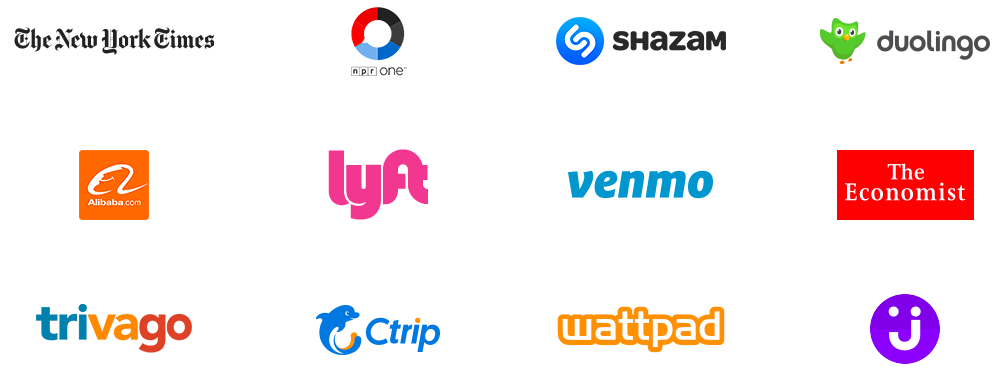
\includegraphics[width=13cm]{Images/chapter2/trusting_apps.png}
		\caption{{\footnotesize Echantaillons des entreprises et applications que utilisent Firebase}}
	\end{center}
\end{figure}

\subsubsection{Facile à intégrer avec Flutter}
Flutter a été créé dans le but de le faire fonctionner sans problème pour Firebase. L'ensemble du processus d'intégration peut prendre jusqu'à 10 minutes, sans qu'il soit nécessaire de fournir beaucoup de données et le processus est totalement simple.\cite{noauthor_using_nodate}

\subsubsection{Tarification flexible}
Firebase offre aux développeurs un modèle de tarification \gls{freemium} flexible et, dans une certaine mesure, généreux, adoptant l’approche consistant à payer à l’échelle de votre application, en commençant par une offre gratuite dans laquelle vous obtenez une quantité limitée de données à stocker et des requêtes de lecture limitées effectuées par pour les applications en croissance, les développeurs peuvent payer un prix fixe pour une utilisation étendue des services de la plate-forme, ainsi que davantage de stockage de données et de requêtes, pour enfin atteindre l'offre illimitée dans laquelle vous êtes facturé pour ce que vous avez utilisé.\cite{noauthor_firebase_nodate}\bigskip

\begin{figure}[h]
	\begin{center}
		
\includegraphics[width=14cm]{Images/chapter2/firebase_pricing_offers.png}
		\caption{{\footnotesize différents modèles de tarification de Firebase}}
	\end{center}
\end{figure}

\section{Google Maps}

\section{Google Books}